\documentclass[10pt]{report}            % Report class in 11 points
\parindent0pt  \parskip10pt             % make block paragraphs
\raggedright                            % do not right-justify
\usepackage{amsmath, amssymb, amsthm,graphicx, enumitem, hyperref,gensymb, float} %, threeparttable}
\usepackage[table]{xcolor}
\newcommand{\ro}{\mathcal{R}_0}
\makeatletter
\newcommand*{\centerfloat}{%
  \parindent \z@
  \leftskip \z@ \@plus 1fil \@minus \textwidth
  \rightskip\leftskip
  \parfillskip \z@skip}
\makeatother
%*******************************************************************%
\title{\bf Mayo Pharmacy Optimization Case Study\\
\large Using Discrete Event Simulation}  % Supply information
\author{Justin Hood\\
MSCS 791}              %   for the title page.
\date{\today}                           %   Use current date.
\begin{document}                        % End of preamble, start of text.
\maketitle                              % Print title page.
\pagenumbering{roman}                   % roman page number for toc
\setcounter{page}{2}                    % make it start with "ii"
%\tableofcontents                        % Print table of contents
\newpage
\section*{Abstract}
\addcontentsline{toc}{section}{Abstract}
\section*{Introduction}                % Print a "chapter" heading\
\addcontentsline{toc}{section}{Introduction}
\pagenumbering{arabic}                  % Start text with arabic 1
Prescription medication is becoming increasingly commonplace in the United States. In 2013, the average number of prescriptions per capita was $12.2$, up from $9$ in 1998 [CITE BOTH]. With this trend in preccription usage on the rise still, pharmacies are becoming an ever greater presence in the lives of americans. As such, pharmacies need to adapt to deal with increasing numbers of orders, as well as increasing the speed and accuracy at which they fill orders, in order to remain competitive in an increasingly saturated landscape of pharmacies.  Consequently, pharmacies must adapt their methodologies and staffing reqirements in order to maximimize the numebr of orders filled and minimize the wait time and employee idle times. Obviously, testing multiple different prioritizations and staffing numbers is both expensive and time consuming, so we shall consider a discrete event simulation approach. In this case study, we are tasked with both modeling and optimizing the workflow for a pharmacy based on samples of data regarding task duration and incoming order frequency. In addition to the sample data for the pharmacy, we are also given a brief overview of the basic workflow for the pharmacy. Using this information, we shall begin by constructing a discrete event simulation in C++ to test our so called ``control" case, i.e. the pharmacy described by the basic information. Once this simulation is running and tested, we shall attack the optimization on two fronts.
\begin{enumerate}
\item Optimizing task priority within the workflow (Picking the best queue to pull from)
\item Optimizing staff breakdown (Best number of pharmacists vs. technicians to employ)
\end{enumerate}
With these optimizations, we should be able to develop a sense of what makes the pharmacy run more efficiently, as well as an idea of what variables could be changed to further increase the accuracy of our simulation, as well as improve the pharmacy's function.
\section*{Background}
\addcontentsline{toc}{section}{Background}
In our prototypical example, there are six basic tasks in the workflow tied to the two different types of orders, oral and IV: order entry, entry verification, oral fill, iv fill, fill verification, and dispensing through the window. In addition to these tasks, there are two different classes of employee [Pharmacist and Technician], who are constrained as to which task they may perform due to both legal regulations as well as potentially company specific guidelines. These regulations dictate that of the tasks, the verification tasks can only be performed by the pharmacists, while the remaining 3 tasks can be performed by both pharmacists and technicians. A breakdown of this hienarchy follows in Table \ref{table:tasks}, with pharmacist specific tasks highlighted in red.
\begin{table}[h]
\centering
\begin{tabular}{|c||c|}
\hline
Technician & Pharmacist\\\hline\hline
Order Entry & Order Entry \\\hline
& \cellcolor{red!25}Entry Verification \\\hline
Drug Preparation & Drug Preparation\\\hline
& \cellcolor{red!25}Preparation Verification\\\hline
Distribution & Distribution\\\hline
\end{tabular}
\caption{Pharmacist vs Technician tasks.}
\label{table:tasks}
\end{table}
The workflow of this pharmacy follows a fairly linear task order as one might expect from the tasks named above, and is illustrated graphically in Figure \ref{fig:flowchart}.
\begin{figure}[h]
\centering
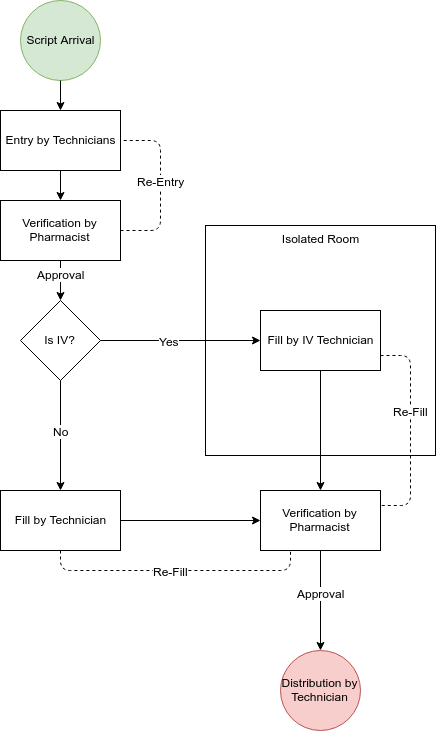
\includegraphics[scale=.5]{Flowchart.png}
\caption{Pharmacy workflow by task position noting which tasks are pharmacist only.}
\label{fig:flowchart}
\end{figure}
We see that the workflow only diverges from being liear at the fill stage of the process, and this is due to the fact that one employee is solely tasked with filling IV orders in isolation.
\section*{Methods}
\addcontentsline{toc}{section}{Methods}
In order to construct our discrete event simulation in C++, we must first identify the basic workflow in the pharmacy. This  This workflow will form the backbone for our simulations main loop. The second stage of development is centered around identifying the distributions from the time sample data provided. In order to run the simulation, we need to know the distributions that each time variable comes from. Finally, we run the simulation and report statistical analysis on the results.
%In order to effectively model and optimize the workflow in this pharmacy, we consider the given scenario, and how we might optimize it. As described, there are essentially no guidelines in place to speed up process workflow, which we will find dramatically affects the overall performance. As a pharmacy, we assume that maximizing both the number of prescriptions and the speed at which they are filled is paramount to the public image as well as its financial success.
\subsection*{Process Workflow}
\addcontentsline{toc}{subsection}{Process Workflow}
To begin, we consider the basic workflow. As stated, due to regulations, pharmacists are able to perform tasks that technicians are unable to. Ignoring the IV technician for the time being as its task is isolated from the main workflow, the task breakdown is as follows:

As illustrated in Table \ref{table:tasks}, we see that pharmacists are capable of doing all steps in the workflow, while the technicians may only perform three of the five. This is to say that $Task_{Technician}\subset Task_{Pharmacist}$.  With this distinction in mind, we consider the flowchart contained in Figure \ref{fig:flowchart}, which describes the process workflow graphically.
\begin{figure}[H]
\centering
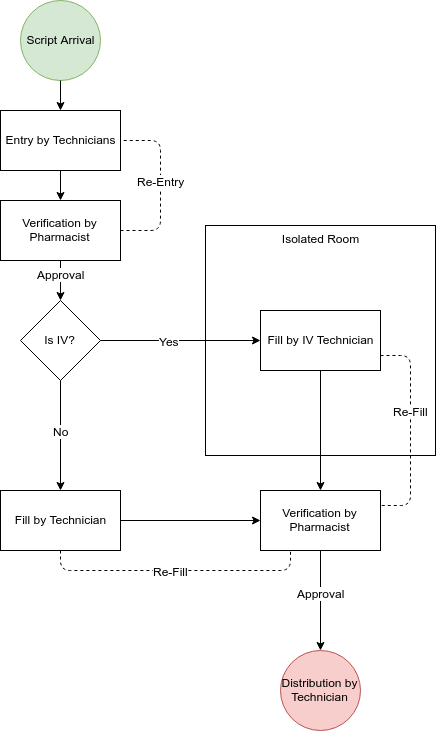
\includegraphics[scale=.5]{Flowchart.png}
\caption{Pharmacy workflow by task position noting which tasks are pharmacist only.}
\label{fig:flowchart}
\end{figure}
Here we may clearly see that with the exception of the IV Fill step, the workflow is fairly linear, which will make the simulation fairly simple in theory, allowing for more advanced optimizations. The basic workflow is:
\begin{enumerate}
\item Order comes in and enters the Entry Task Queue
\item Employee enters the order, order enters the Entry Verification Queue
\item Pharmacist verifies the entry, order enters the Fill Queue
\item Employee fills the order, order enters the Fill Verification Queue
\item Pharmacist verifies the fill, order enters the Dispense Queue
\item Employee dispenses the order through the window
\end{enumerate}
There is a fork in the process workflow after step 3, where the order's type (Oral vs. IV) must be checked so it may be put in the appropriate filling queue, however this does not affect the linearity of the process at this step. With this workflow defined, we consider the next step of building our simulation, identifying the distributions from which we sample times from.
\section*{Distribution Identification}
\addcontentsline{toc}{section}{Distribution Identification}
As we have identified in the workflow above, there are essentially six pivotal points that will have times associated with them: Entry, Entry Verification, Oral Drug Preparation, IV Drug Preparation, Order Prep Verification, and Distribution. In addition to these six points, we are also aware of the fact that the times between incoming oral and IV orders come from different distributions. As part of the given data, we have a sample of the times from each of these eight different categories, ranging in size from 34 to 60 observations. Using each of these samples, we shall construct Cullen and Frey graphs to attempt to isolate the correct distributions. With this set of hypothetical distributions in hand, we shall fit the data and test the goodness of fit statistic to identify the best fit.
\subsection*{Order Entry}
\addcontentsline{toc}{subsection}{Order Entry}
To begin, we consider the data provided for the order entry times. Using $R$, we construct both a histogram and a Cullen and Frey graph (Figure \ref{fig:orderEntryHistCullen}),
\begin{figure}[H]
\centering
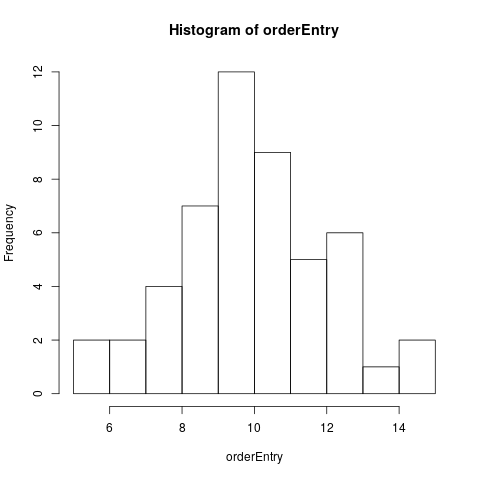
\includegraphics[scale=.35]{OrderEntryHist.png}
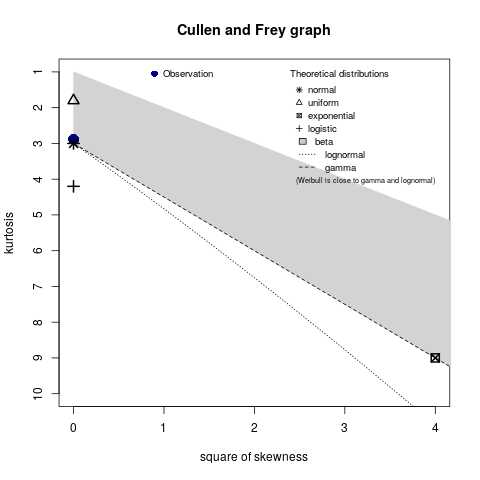
\includegraphics[scale=.35]{OrderEntryCullen.png}
\caption{Histogram of order entry times (left) and its corresponding Cullen and Frey graph (right)}
\label{fig:orderEntryHistCullen}
\end{figure}
Looking at these plots, it appears that the data comes from a normal population, and the Cullen and Frey plot supports this. For completeness, we shall test this sample as being from a normal distribution as well as a gamma and log-normal distribution. Once the data has been fit with each of these distributions, $R$ is used to compute a goodness of fit statistic for each model, and these results follow:
\begin{table}[H]
\centerfloat
\begin{tabular}{|r||c|c|c|}
\hline
& Normal Fit & Gamma Fit & log-normal Fit \\\hline
Kolomogorov-Smirnov & \cellcolor{green!25}0.05172573 & 0.07123761 & 0.08600921\\\hline
Anderson Darling & \cellcolor{green!25}0.14921512 & 0.28840960 & 0.45314418\\\hline
AIC & \cellcolor{green!25}219.8769 & 221.3501 & 223.2712\\\hline
\end{tabular}
\caption{Goodness-of-Fit statistics for hypothetical fits on the order entry data.}
\label{table:entryGOF}
\end{table}
As highlighted in Table \ref{table:entryGOF}, by treating this sample as part of a larger normal population, we produce the smallest goodness-of-fit statistics, implying the best fit. As such, we shall treat this as the correct distribution for sampling purposes in our simulation. The relevant distribution statistics follow,
\[\text{Order Entry}\sim N(\mu=9.873784,\ \sigma=2.095579)\]
\subsection*{Remaining Distributions}
\addcontentsline{toc}{subsection}{Remaining Distributions}
In a similar fashion, the remaining distributions are identified as follows:
\begin{align*}
\text{Entry Verification Times} &\sim U(1.2726,\ 3.4059)\\
\text{Oral Preparation Times} &\sim \text{Lognormal}(\mu=2.99140489,\ \sigma=.06300657)\\
\text{IV Preparation Times} &\sim \text{Weibull}(shape=2.362195,\ scale=6.359247)\\
\text{Preparation Verification Times} &\sim \text{Weibull}(shape=2.911269,\ scale=2.143830)\\
\text{Dispense Times} &\sim N(\mu=2.947898,\ \sigma=0.566620)\\
\text{Oral Incoming Times} &\sim \text{Exponential}(\lambda = 0.129199 )\\
\text{IV Incoming Times} &\sim \text{Exponential}(\lambda = 0.05988024 )
\end{align*}
With these distributions in hand, we can begin the construction of the base case of the simulation.
\section*{First Layer of Optimization}
\addcontentsline{toc}{section}{First Layer of Optimization}
To begin our two pronged optimization efforts, we begin by trying to improve the task logic. To begin we model the base case.
\subsection*{Construction of the Base Case}
\addcontentsline{toc}{subsection}{Base Case}
To construct the simulation of the pharmacy, the programming language C++ was used due to its speed, as well as object oriented structure. This structure allowed for maximal customization of our data. To build the simulation, two unique class objects were written to house the details required for a given order, as well as each of the employees. Within these classes relevant structures for computing the idle times and other important statistics are included and updated throughout the simulation. An outline of the pseudo-code for the simulation follows:
\begin{verbatim}
Read in user input (number of hours, sampling frequency, number of employees, etc.)
For(each simulation){
    Construct workers and place in idle pool
    Calculate relevant duration times in queues from distribution data
    while(!endOfSim){
        Check and see if new order enters in this time step
        Check if any active workers have finished task
        if(Finished){
            Push order to next queue, move employee to idle pool
        }else{
            Increment time step
        }
        For(each idle worker){
            if(any queue not empty){
                Assign task at random                   
            }else{
                Add to idle time
            }
        }
        Write queue lengths to file
    }
    Write end of simulation data
}
\end{verbatim}
With this simulation constructed, the base case was run using the following parameters,
\begin{itemize}
\item Number of Hours: 12
\item Number of Updates per Minute: 4 (Every 15 seconds)
\item Number of Pharmacists: 2
\item Number of Techs: 5 (4 Normal and 1 IV)
\item Number of Trials: 30
\end{itemize}
It is important to note here the job assignment of the base case. In this model, when job assignment begins for each employee, each non-empty job is put into a pool and randomly chosen with no priority. So, a pharmacist has an equal probability of doing a pharmacist only task or a technician level task. Changing this assignment will become a cornerstone of our optimization efforts.
\subsubsection*{Base Case Results}
Using the parameters above, the following 95\% confidence intervals were obtained,
\begin{align*}
\text{Oral Incoming} &= [91.6024,\ 98.06426] && \text{Number of Orders}\\
\text{IV Incoming} &= [42.47068,\ 47.12932] && \text{Number of Orders}\\\\
\text{Entry Queue} &= [0.4310875,\ 0.6114125] && \text{Number of Orders}\\
\text{Entry Verification Queue} &= [7.997571,\ 12.58185] && \text{Number of Orders}\\
\text{Oral Fill Queue} &= [0.1240198,\ 0.1679247] && \text{Number of Orders}\\
\text{IV Fill Queue} &= [0.079518,\ 0.1349264] && \text{Number of Orders}\\
\text{Fill Verification Queue} &= [3.427384,\ 5.809907] && \text{Number of Orders}\\
\text{Dispense Queue} &= [0.1735777,\ 0.2304964] && \text{Number of Orders}\\\\
\text{Oral Filled} &= [67.26063,\ 70.40604] && \text{Number of Orders}\\
\text{IV Filled} &= [32.72671,\ 37.33995] && \text{Number of Orders}\\\\
\text{Pharmacist Idle Time} &= [2.811366,\ 4.692106] && \text{Percent of Total Time}\\
\text{Technician Idle Time} &= [17.50725,\ 20.02053] && \text{Percent of Total Time}\\
\text{IV Technician Idle Time} &= [67.62806,\ 71.53167] && \text{Percent of Total Time}\\\\
\text{Oral Throughput Times} &= [105.1253,\ 136.618] && \text{Minutes}\\
\text{IV Throughput Times} &= [91.9162,\ 127.0587] && \text{Minutes}\\
\text{Oral Wait Times} &= [68.11842,\ 99.61155] && \text{Minutes}\\
\text{IV Wait Times} &= [69.27191,\ 104.3281] && \text{Minutes}\\\\
\end{align*}
While these intervals do provide important analysis on the data, a graphical interpretation of this data will help us to more accurately examine potential points of congestion in the model. Figure \ref{fig:baseQ} has box and whisker plots for each of the queues in the base case.
\begin{figure}[H]
\centering
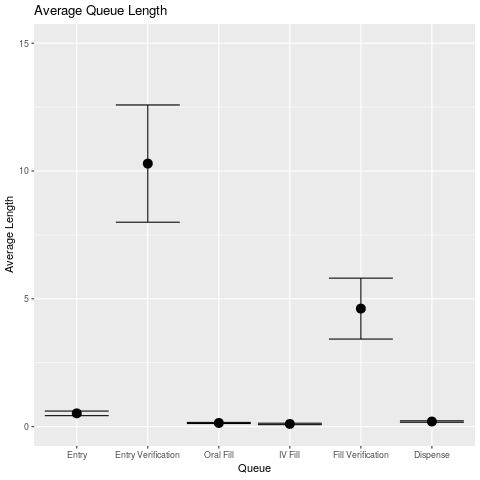
\includegraphics[scale=.5]{BaseQueueCIs.png}
\caption{Box and whisker plots for average queue lengths by type}
\label{fig:baseQ}
\end{figure}
We see that the results of this simulation point to the verification queues as being congestion points. Notably, these are the two tasks in the workflow that are pharmacist specific. This congestion then is likely due to the method by which workers received their job assignments. With the pharmacists choosing from all possible tasks equally, they can take work from the technicians, who cannot in return work from the verification tasks. Reducing this congestion will be the goal of our first optimization.
*******Talk about idle times*******************
\subsection*{First Optimization: Lazy Pharmacists}
\addcontentsline{toc}{subsection}{Lazy Pharmacists}
Given that the verification tasks are causing congestion in the base model, we consider the effects of changing the job assignment method in the simulation to the following.
\begin{verbatim}
if(pharmacist){
    if(verification queues !empty){
        choose one at random
    }else{
        do nothing
    }
}
if(technician){
    if(any queues !empty){
        choose one at random
    }else{
        do nothing
}
\end{verbatim}
Under this scheme, the pharmacists will only do pharmacist specific tasks, leaving the technicians to do the remainder of the tasks. Running the simulation with the same parameters as the base case, under the new job choice logic yields some unexpected results. Firstly, the average queue lengths are much different. Figure \ref{fig:basevprof} shows the differing results.
\begin{figure}[H]
\centering
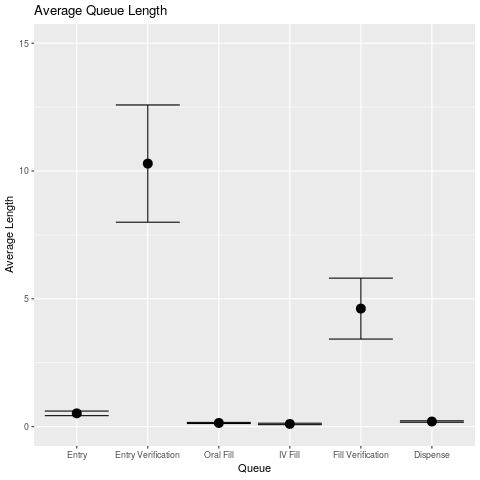
\includegraphics[scale=.35]{BaseQueueCIs.png}
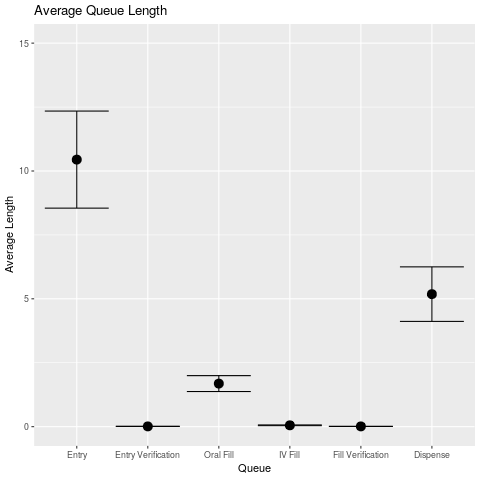
\includegraphics[scale=.35]{ProfQueueCIs.png}
\caption{Base case (left) vs. Lazy Pharmacist (Right) average queue lengths}
\label{fig:basevprof}
\end{figure}
Under the original schema, all queues were essentially empty except for the verification queues, while under our new schema all of the non-verification queues show increases. Indeed we find that the average queue length for our new case is slightly larger than before,
\[\overline{Length}_{Base}=2.648<2.898=\overline{Length}_{Lazy Pharmacist}\]
In addition to this, the average idle time for an employee is significantly larger,
\[\overline{Idle}_{Base}=14.475\% < 21.627\%=\overline{Idle}_{Lazy Pharmacist}\]
Looking more closely into this idle time data, we see that the average idle time for a pharmacist in the new scheme is approximately $67\%$, which is clearly not an effective use of their time. As such, we seek to find a better process optimization.
\subsection*{Second Optimization: Largest Queue}
\addcontentsline{toc}{subsection}{Largest Queue}
Given that forcing the pharmacists to only pull from the verification tasks is hurting the efficiency of the model, we consider a new job assignment logic, choosing the largest possible task. So, a pharmacist will choose to take their next task from the largest of all 5 possible queues, while technicians may choose from the 3 technician level queues. Running the simulation with the same parameters as the base case, under the new job choice logic yields results that are more aligned with what we would expect. Figure \ref{fig:basevlong} shows the comparison on average queue lengths between the base case and the longest queue method.
\begin{figure}[H]
\centering
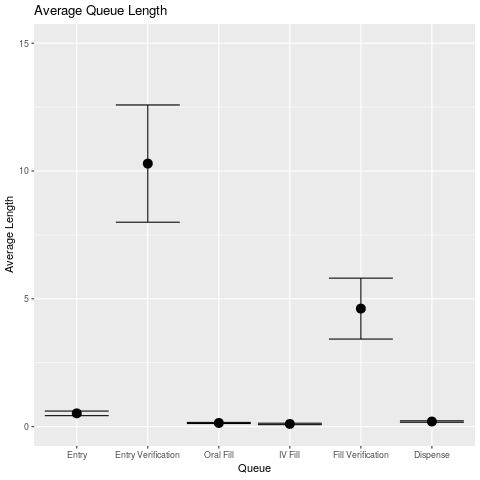
\includegraphics[scale=.35]{BaseQueueCIs.png}
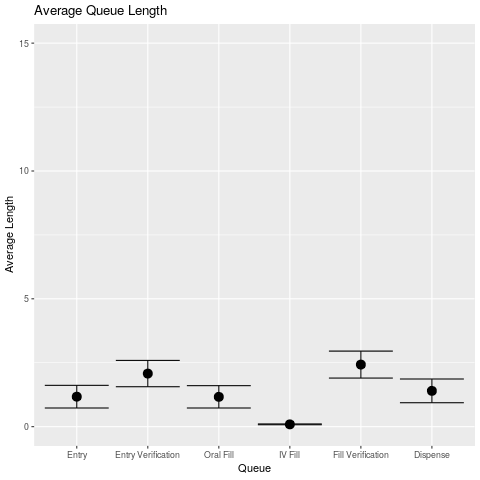
\includegraphics[scale=.35]{LongestQueueCIs.png}
\caption{Base case (left) vs. Largest Queue (Right) average queue lengths}
\label{fig:basevlong}
\end{figure}
We see that under this new system, all of the queues (except IV fill) have non-zero means, but that they are all relatively small compared to the mean of approximately 10 for the base entry verification length. Looking deeper into the data, we see that the average queue length is reduced from $2.648$ in the base case to $1.389$ in this new method. In addition to this, average idle time for the workers is reduced from $14.475\%$ in our base model to $13.395\%$. While these changes may seem somewhat small, consider now the mean throughput times between the two models.
\begin{figure}
\centering
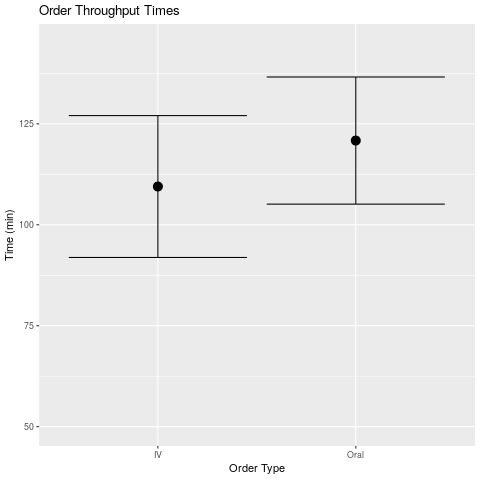
\includegraphics[scale=.35]{BaseThroughputCIs.png}
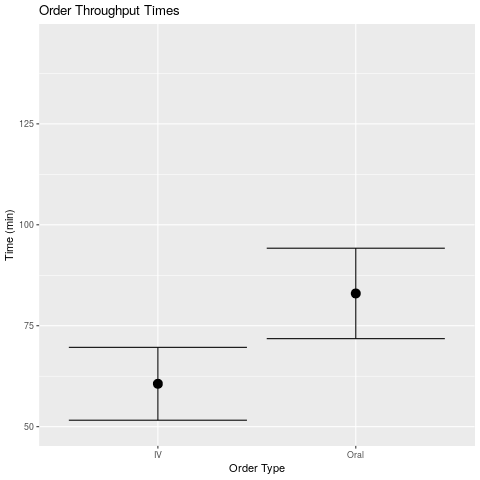
\includegraphics[scale=.35]{LongestThroughputCIs.png}
\caption{Base case (left) vs. Largest Queue (Right) average throughput times by order type}
\label{fig:basevlongthrough}
\end{figure}
We see that by choosing the longest queue as the next task, the average throughput time for an order is reduced by a factor of almost $30\%$, which seems fairly significant. While this method is clearly superior to the base case, we consider finally a combination of the Lazy Pharmacist and Longest Queue methods.
\subsection*{Third Optimization: Smart Method}
\addcontentsline{toc}{subsection}{Smart Method}
As our final job assignment optimization we consider a sort of mixture between choosing the longest queue, and relegating the pharmacists to the verification queues. Namely, under this schema, the pharmacist will first check to see if any of the verification queues are non-empty, and if so, they will choose the largest one. Otherwise, they choose the largest from the remaining queues. The technicians remain unchanged from before.
\begin{verbatim}
if(pharmacist){
    if(either verification queue is nonempty){
        choose largest
    }else{
        choose largest technician level queue
    }
}
if(technician){
    choose largest technician level queue
}
\end{verbatim}
Again we implement this model with the basic parameters from before, getting again better results than before. Since we have established that the longest queue is our front-runner for the optimization, we shall use it as a basis for comparison for this smart method. First, we compare the base queue lengths,
\begin{figure}[H]
\centering
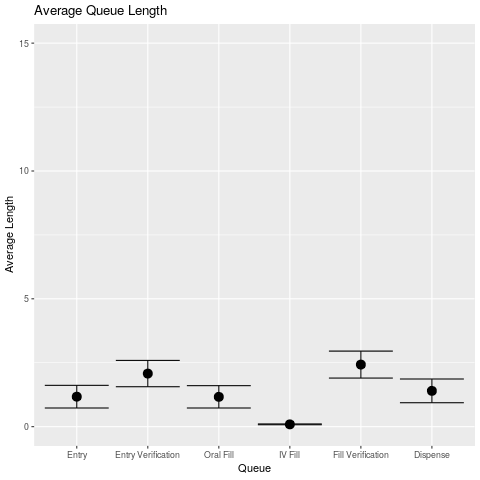
\includegraphics[scale=.35]{LongestQueueCIs.png}
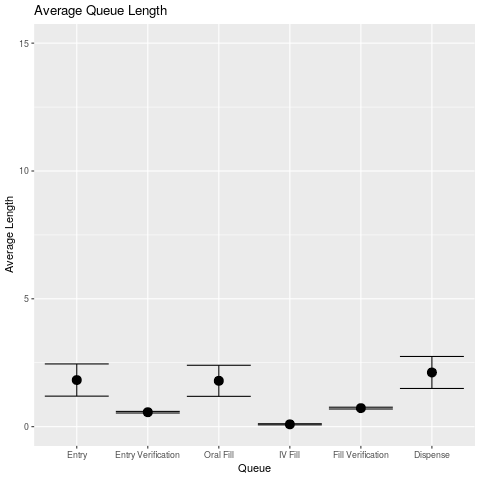
\includegraphics[scale=.35]{SmartQueueCIs.png}
\caption{Largest Queue (left) vs. Smart Method (Right) average queue lengths}
\label{fig:longvsmart}
\end{figure}
As expected based on the results of the lazy pharmacist method, we see improvement in the size of the verification queue lengths at the slight cost to the remainder of the queue lengths. Looking into the data we find,
\[\overline{Length}_{Longest}=1.389 > 1.187 = \overline{Length}_{Smart}\]
\[\overline{Throughput}_{Longest}=71.813 > 64.920 = \overline{Length}_{Smart}\]
It would appear that we have achieved a slight increase in effectiveness with this new implementation, but it is hard to say given the relative magnitudes of the standard deviations in the data, thus further analysis is required.
\section*{Comparing the First Stage Optimizations}
\addcontentsline{toc}{section}{Comparing First Stage Optimizations}
Given that a pharmacy is a business above all else, the goal of these optimizations should be to increase the number of orders filled and reduce the employee idle times as much as possible. As such, we shall conduct a one-way ANOVA test on the mean number of orders filled to find the most effective model under the given conditions. Looking first at the IV filled data across the different methods, we see no marked difference among the four, they are all within one standard deviation of each other. As such, we shall focus on the oral filled data, as there is more significant variation in the results. First, let us consider a collation of the oral filled data across the methods, Table \ref{table:collate}.
\begin{table}[H]
\centerfloat
\begin{tabular}{|r||c|c|c|}
\hline
Method & Mean & Standard Deviation & $n$\\\hline\hline
Base Case & $68.8$ & $4.40$ & $30$\\\hline
Lazy Pharmacist & $61.7$ & $4.85$ & $30$\\\hline
Largest Queue & $73.3$ & $9.18$ & $30$\\\hline
Smart Method & $78.4$ & $6.04$ & $30$\\\hline
\end{tabular}
\caption{Collation of the Oral Fill data for each of the different optimization methods}
\label{table:collate}
\end{table}
While Table \ref{table:collate} allows us to see the numbers, it is more useful to see the difference in a graphical form as in Figure \ref{fig:anovaBox}.
\begin{figure}[H]
\centering
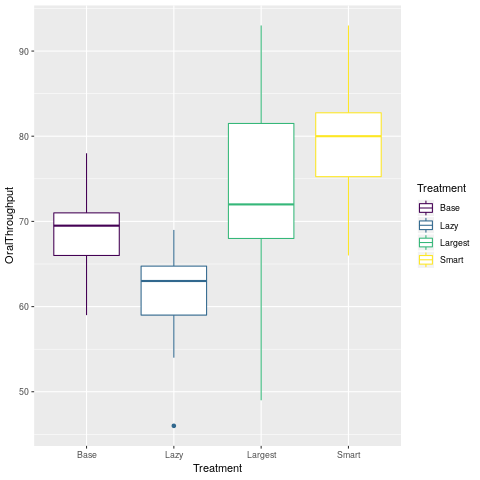
\includegraphics[scale=.5]{anovaBox.png}
\caption{Box plots for the Oral Fill data in each method}
\label{fig:anovaBox}
\end{figure}
We see from Figure \ref{fig:anovaBox} that there does seem to be a difference among the models, though it is hard to confirm visually. Running the ANOVA test on the null hypothesis of $\mu_i=\mu_j\ \forall i,j\in\text{Methods}$, we arrive at the $F$ statistic, $F=36.96\Rightarrow p<2\times10^{-16}$, which is highly significant. Given this $p$ value, we reject the null hypothesis in favor of the alternative, that there is a difference in at least one of the means. Given this result, we shall use $R$ to compute the Tukey honest significant differences between the means, whose results can be found in Table \ref{table:tukey}.
\begin{table}[H]
\centerfloat
\begin{tabular}{|r||c|c|}
\hline
Methods & Difference & $p$-value\\\hline\hline
Lazy-Base   &  $-7.133333$ & $0.0001922$\\\hline
\cellcolor{yellow!25}Largest-Base  & \cellcolor{yellow!25}$4.500000$ & \cellcolor{yellow!25}$0.0367813$\\\hline
Smart-Base  &   $9.600000$ & $0.0000003$\\\hline
Largest-Lazy & $11.633333$ & $0.0000000$\\\hline
Smart-Lazy  &  $16.733333$ & $0.0000000$\\\hline
\cellcolor{yellow!25}Smart-Largest & \cellcolor{yellow!25}$5.100000$ & \cellcolor{yellow!25}$0.0132541$\\\hline
\end{tabular}
\caption{Tukey HSD for different method means}
\label{table:tukey}
\end{table}
Note, Table \ref{table:tukey} has two rows highlighted. These rows correspond to the differences between the base method and largest queue method, as well as the largest queue method to the smart method. Based on the table, we can draw the following conclusion comparing the different methods,
\[\text{Smart $>$ Largest $>$ Base}\]
Now that we have established an ``optimal" method, we now consider how best to improve efficiency in employees.
\section*{Efficiency Mesh}
\addcontentsline{toc}{section}{Efficiency Mesh}
Up until this point, all of our analysis has been performed on the basic assumptions from the base case,
\begin{itemize}
\item Number of Hours: 12
\item Number of Updates per Minute: 4 (Every 15 seconds)
\item Number of Pharmacists: 2
\item Number of Techs: 5 (4 Normal and 1 IV)
\item Number of Trials: 30
\end{itemize}
While this may be the current conditions of the pharmacy, it is still possible that this is not the most cost effective staffing. In order to determine the best possible configuration of employees, we shall construct a $10\times 10$ mesh that defines the pharmacies profit as a function of the number of employees of each type. Here, each point in our mesh corresponds to a coordinate in the Technician-Pharmacist plane that has a magnitude of profit. In order to assure fairness, the simulation is run with the same input sampling for each step, and run 30 times to allow for random variance in choosing queues to be accounted for. Let us define the profit function as,
\[\mathcal{P}=\$55.99(Filled_{Oral}+Filled_{IV})-\$748.92(n_{Pharmacist})-\$63.12(n_{Technician})\] **********Cite money************\\
That is to say, the pharmacy profit for a given employee configuration is revenue per filled order times the number of filled orders less the cost of employees in the configuration. Using the Smart Method developed earlier, we create a 3-D surface that describes the profit. A 2-D heat-map projection of profit appears in Figure \ref{fig:heatmap}.
\begin{figure}[h]
\centering
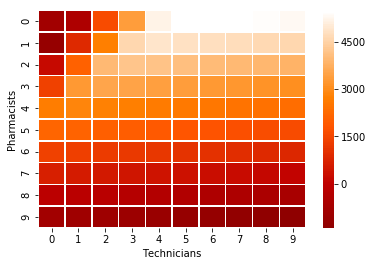
\includegraphics[scale=.75]{profitheatmap.png}
\caption{Heatmap of profit values using the Smart Method. Note, labeling on the $x$ and $y$ axes is reduced by one due to indexing.}
\label{fig:heatmap}
\end{figure}
As evidenced by the heat map, we see that the most profitable configurations occur for low numbers of pharmacists and higher numbers of technicians to compensate.  In fact, we find that the optimal numbers of employees for this test is one pharmacist and seven technicians (6 normal and 1 IV). This resulted in a net profit, $\mathcal{P}(1,7)=\$5488.85$, though most of the surrounding mesh points had an approximately similar value, at least in the technician direction.\\
This being said, there are a number of issues with this efficiency mesh. It makes broad assumptions about the value of each filled order, which could obviously be fixed using real data that the pharmacy would be able to provide.
\section*{Conclusions}
\addcontentsline{toc}{section}{Conclusions}
After performing both layers of optimization, we see that there is a large range of efficiencies possible for this pharmacy. As we found before, simple workflow management methods could be implemented to reduce average throughput time by nearly a third, as well as reduce employee idle times...\\
Note about skill efficiencies and dispositions, as well as leftovers from before, long term running ideas.
%\subsection*{SIR Model}
%\addcontentsline{toc}{subsection}{SIR Model}
%
%\subsection*{Beta}
%\addcontentsline{toc}{subsection}{Beta}
%$\beta$ is a product of many factors, the main being team success, physical locale (weather, population, income), and the social environment of the city\cite{light}. In order to compute a given teams $\beta$ value, we must quantify these factors as follows.
%\subsubsection*{Team Success}
%\addcontentsline{toc}{subsection}{Team Success}
%
%\begin{equation}\label{acoeff}
%\log(a_t) = 14.1 + 0.2205(WINT)+.091\log(POP)-0.3766\log(INC)
%\end{equation}
%\begin{equation}\label{bcoeff}
%\log(b_t) = 9.171 + .03(WINT)+.028\log(POP)-.1879\log(INC)
%\end{equation}
%Each of the coefficients we compute have incredibly large t-values, which aligns with the linear nature of (\ref{a}) and (\ref{b}). As such, we are confident that these coefficients are correct for the purposes of our analysis. With these coefficients computed, we can compute the following location score for our potential Milwaukee team,
%
%\begin{table}[H]
%\centerfloat
%\begin{tabular}{lrrrrrrrr}
%\hline
%\multicolumn{9}{c}{Location Score for Milwaukee} \\
%Team & Population$^a$ & GDP per capita$^b$ & Temperature$^c$ & WINT & $a_t$ & $b_t$ & $H_t$ & $h_t$\\
%\hline
%Milwaukee & 1.572245 & \$58,680.00 & -2 & 1 & 27583.4 & 1274.342 & 117.1288 & 0.9990123
%\end{tabular}
%\caption{$^a$in Millions \cite{population}; $^b$USD \cite{gdp}; $^c$ \degree C \cite{weather}}
%\label{table:Milwaukee_H}
%\end{table}
%
%\end{description}
\begin{thebibliography}{9}
%\bibitem{light} J. Light, A. Chernin, and J. M. Heffernan, ``NHL expansion and fan allegiance: a mathematical modelling study,” \textit{Mathematics-in-Industry Case Studies}, vol. 7, no. 1, Apr. 2016.
%\bibitem{money} M. Ozanian and K. Badenhausen, ``The NHLs Most Valuable Teams” \textit{Forbes}, 21-Feb-2019. [Online]. Available: \url{https://www.forbes.com/sites/mikeozanian/2018/12/05/the-nhls-most-valuable-teams/}. [Accessed: 25-Sep-2019].
%\bibitem{stats}  HockeyDB.com (2019) National Hockey League history and statistics. \url{http://www.hockeydb.com/ihdb/stats/leagues/141.html}. Web
%\bibitem{jones}J. C. H. Jones and D. G. Ferguson, ``Location and Survival in the National Hockey League,” \textit{The Journal of Industrial Economics}, vol. 36, no. 4, p. 443, Jun. 1988.
%\bibitem{population} US Census Bureau and Data Integration Division, ``Population Estimates,” \textit{Metropolitan and Micropolitan Statistical Area Totals Dataset: Population and Estimated Components of Change: April 1, 2010 to July 1, 2014 - U.S Census Bureau}. [Online]. \url{https://web.archive.org/web/20150504102404/http://www.census.gov/popest/data/metro/totals/2014/CBSA-EST2014-alldata.html}. [Accessed: 30-Sep-2019].
%\bibitem{gdp} ``Regional Economic Accounts GDP and Personal Income,” \textit{BEA}. [Online]. \url{https://apps.bea.gov/itable/drilldown.cfm?reqid=70&stepnum=40&Major_Area=5&State=5&Area=XX&TableId=504&Statistic=1&Year=2014&YearBegin=-1&Year_End=-1&Unit_Of_Measure=Levels&Rank=1&Drill=1&nRange=5}. [Accessed: 28-Sep-2019].
%\bibitem{weather} ``Milwaukee Temperatures: Averages by Month,” \textit{Milwaukee WI Average Temperatures by Month - Current Results}. [Online]. \url{https://www.currentresults.com/Weather/Wisconsin/Places/milwaukee-temperatures-by-month-average.php}. [Accessed: 30-Sep-2019].
%\bibitem{whynot} J. Hand, C. Jozwik, H. Magner, Z. Brooke, A. Landowski, A. Parquette, and E. Johnson, ``Why Milwaukee is Not an NHL City,” \textit{Milwaukee Magazine}, 16-Nov-2018. [Online]. \url{https://www.milwaukeemag.com/milwaukee-not-nhl-city/}. [Accessed: 29-Sep-2019].
%\bibitem{draft} ``2017 NHL Expansion Draft,” \textit{Wikipedia}, 27-Apr-2019. [Online]. \url{https://en.wikipedia.org/wiki/2017_NHL_Expansion_Draft}. [Accessed: 29-Sep-2019].
%\bibitem{wisco} ``NHL Players Born in Wisconsin, United States,” \textit{Hockey}. [Online]. \url{https://www.hockey-reference.com/friv/birthplaces.cgi?country=US&province&state=WI&fbclid=IwAR1vb6vzR95-DX0B_zRyV_gLxYcWMneos3Ppn8RBNsnHQqzA9d4sJj4X_aA}. [Accessed: 29-Sep-2019].
\end{thebibliography}
\end{document}                          % The required last line
